\section{Prediction error}

To assess prediction quality, we define the prediction error (or residual) as:
\[\varepsilon(t+r)=v(t+r)-\hat{v}(t+r|t)\]
The optimal predictor minimizes the mean square prediction error (MSPE), which is the variance of the residual:
\[\min\left( \mathbb{E}\left[\varepsilon(t)^2 \right] \right)\]
Recalling the expansion of $W(z)$ in negative powers of $z$: 
\[W(z)=w_0+w_1z^{-1}+w_2z^{-2}+\dots\]
We can express $v(t)$ as an infinite linear combination of past noise values:
\[v(t)=w_0\eta(t)+w_1\eta(t-1)+w_2\eta(t-2)+\dots\]
Suppose the past of $\eta(\cdot)$ is measured. 
Then, we could use this information to estimate $v(t+r)$ for $r \geq 1$: 
\[v(t+r)=\underbrace{w_0\eta(t+r)+w_1\eta(t+r-1)+\dots+w_{r-1}\eta(t+1)}_{\alpha(t)} +\underbrace{w_r\eta(t)+w_{r+1}\eta(t-1)+\dots}_{\beta(t)} \]
Now, $\alpha(t)$ and $\beta(t)$ are uncorrelated random variables (they are linear combinations of the same white noise process over non-overlapping time ranges):
\begin{itemize}
    \item $\beta(t)$ can be computed once the past of $\eta(\cdot)$ (up to $t$) is known. 
    \item $\alpha(t)$ depends on the future of $\eta(\cdot)$ (from $t+1$ to $t+r$). 
\end{itemize}
Thus, $\alpha(t)$ exhibits no correlation with the past until time $t$, indicating its unpredictability based on past information. 
Consequently, we can solely estimate its mean, which is zero:
\[\mathbb{E}=w_0\mathbb{E}\left[\eta(t+r)\right]+w_1\mathbb{E}\left[\eta(t+r-1)\right]+\dots+w_{r-1}\mathbb{E}\left[\eta(t+1)\right]=0\]
This leads to the optimal predictor:
\[\hat{v}(t+r|t)=\beta(t)=w_r\eta(t)+w_{r+1}\eta(t-1)+\dots\]
The prediction error is then given by:
\[\varepsilon(t+r)=v(t+r)-\hat{v}(t+r|t)=\alpha(t)=w_0\eta(t+r-1)+\dots+w_{r-1}\eta(t+1)\]
It's notable that $\varepsilon(\cdot)$ represents a Moving Average (MA) process. 
Its mean value is 0, and its variance is $(w_0^2 + w_1^2 + \dots + w_{r-1}^2)\lambda^2$.

Moreover, the variance increases monotonically with $r$, signifying that prediction uncertainty escalates with the prediction horizon:
\begin{itemize}
    \item For $r=1$, the variance equals $w_0^2\lambda^2$. 
        When $w_0=1$ (if the function $W(z)$ is canonical), it aligns with the noise variance:
        \[\text{Var}\left[\varepsilon(t) \right]=\text{Var}\left[\eta(t) \right]\]
    \item As $r$ approaches infinity, the variance becomes $(w_0^2 + w_1^2 + \dots)\lambda^2$, equivalent to the variance of the entire process $v(t)$:
        \[\text{Var}\left[\varepsilon(t) \right]=\text{Var}\left[v(t) \right]\]
\end{itemize}
Indeed, prediction becomes progressively challenging with increasing $r$ since the estimation pertains to a distant time point beyond the available data. 
Over time, past data lose their utility, and the most reasonable estimate is the variable's mean: 
\[\mathbb{E}\left[v(t+r)\right]=0\]
Consequently, the variance of the prediction error approaches that of the process:
\[\text{Var}\left[\varepsilon(t)\right]=\mathbb{E}\left[\left(v(t+r)-\hat{v}(t+r|t)\right)^2\right]=\text{Var}\left[v(t)\right]\]
The optimal predictor can be expressed using operator notation:
\[\hat{v}(t+r|t)=\left[w_r+w_{r+1}z^{-1}+w_{r+2}z^{-2}+\dots \right]\eta(t)=\hat{W}_r(z)\eta(t)\]
To determine $\hat{W}_R(z)$, observe that the transfer function can be expressed as:
\begin{align*}
    W(z)    &= w_0+w_1z^{-1} + \dots + w_{r-1}z^{-(r-1)}+w_rz^{-r}+w_{r+1}z^{-r-1}+\dots \\
            &= \underbrace{\left(w_0+w_1z^{-1} + \dots + w_{r-1}z^{-(r-1)}\right)}_{E(z)}  +z^{-r}\underbrace{\left( w_r+w_{r+1}z^{-1}+\dots\right)}_{\hat{W}_r(z)} \\
            &= E(z)  +z^{-r}\hat{W}_r(z)              
\end{align*}
Where $E(z)$ is a polynomial of degree $r-1$, and $\hat{W}_r(z)$ is a power series in $z^{-r}$ (equal to a transfer function). 
Thus, $\hat{W}_r(z)$ can be determined operating the long division of the numerator of $W(z)$ by its denominator performed for $r$ steps: 
\[\hat{W}_r(z)=\dfrac{F_r(z)}{A(z)}\]
Where $F_r(z)$ is the remainder of the division. 
\begin{example}
    Consider the AR(1) process: 
    \[v(t)=av(t-1)+\eta(t)\quad \eta(cdot)\sim WN(0,\lambda^2)\]
    Let's perform the long division on the transfer function for three steps. 
    We obtain: 
    \begin{align*}
        \hat{W}_1(z)=\dfrac{a}{1-az^{-1}} \qquad \lambda_\varepsilon^2=\lambda^2 \\
        \hat{W}_2(z)=\dfrac{a^2}{1-az^{-1}} \qquad \lambda_\varepsilon^2=(1+a^2)\lambda^2 \\ 
        \hat{W}_3(z)=\dfrac{a^3}{1-az^{-1}} \qquad \lambda_\varepsilon^2=(1+a^2+a^4)\lambda^2
    \end{align*}
    For a generic prediction horizon $r$, one gets: 
    \[\hat{W}_r(z)=\dfrac{a^r}{1-az^{-1}} \qquad \lambda_\varepsilon^2=(1+a^2+a^4+\dots+a^{2(r-1)})\lambda^2\]
    For $r$ that tends to infinity $a^r$ tends to zero, and, consequently $\hat{v}(t+r|t)=0$. 
    Moreover, since $\left\lvert a\right\rvert  < 1$, the variance of the residual equals 
    \[\lambda_{\varepsilon}^2=\sum_{i=0}^\infty a^{2i}=\sum_{i=0}^\infty (a^2)^{i}=\dfrac{1}{1-a^2}\]
    Which coincides with the variance of the process $\text{Var}\left[v(t)\right]$. 

    The optimal 1-step ahead predictor is given by:
    \[\hat{v}(t+1|t)=\hat{W}_1\eta(t)=\dfrac{a}{1-az^{-1}}\eta(t)=a\hat{v}(t|t-1)+a\eta(t)\]
    The prediction error equals $\varepsilon(t) = v(t) +\hat{v}(t|t-1)$ and its dynamics are obtained by subtracting the predictor equation from the model equation:
    \[v(t+1)- \hat{v}(t+1|t) = av(t) + \eta(t+1) - a\hat{v}(t|t-1) - a\eta(t) \qquad \varepsilon(t+1) = a\varepsilon(t) + \eta(t+1) - a\eta(t) \]
    Then, the variance of the prediction error can be calculated as: 
    \[\text{Var}\left[\varepsilon(t+1)\right]=\text{Var}\left[\varepsilon(t)\right]=\lambda^2\]
    Notice that the predictor:
    \[\hat{v}(t+1|t)=v(t)\]
    is not optimal. 
    Indeed, 
    \[\varepsilon(t+1)=v(t+1)-\hat{v}(t+1|t)=v(t+1)-v(t)\]
    We can obtain that: 
    \[\mathbb{E}\left[ \varepsilon(t+1)^2 \right]=\dfrac{2}{1+a}\lambda^2\]
    Now, since $\left\lvert a\right\rvert  < 1$, the MSPE of the trivial predictor is larger than that associated with the optimal predictor. 
\end{example}
The optimal predictor that we have determined depends on past values of the white noise process.
However, these are not generally available: we typically have a sequence of data of the $v(\cdot)$ process only. 
Assume that:
\begin{itemize}
    \item $W(z),\eta(t)$ is a canonical representation of $v(t)$. 
    \item $W(z)$ has no zeros on the unit circle boundary ($\Sigma(\omega)>0 \quad \forall\omega$). 
\end{itemize}
Then, we can recover $W(t)$ using a whitening filter (with transfer function $W(z)^{-1}$): 
\[\eta(t)=\dfrac{A(z)}{C(z)}v(t)\]
The whitening filter provides a well-defined representation of $\eta(t)$, since polynomials $A(z)$ and $C(z)$ have the same degree, and therefore $\check{W}(z) = W(z)^{-1}$ can rightfully be interpreted as a transfer function, and, besides, $C(z)$ is a Schur-stable polynomial, which guarantees the stationarity of the process. 
Combining the whitening filter with the optimal predictor from the noise, we obtain the optimal predictor from the process data: 
\begin{figure}[H]
    \centering
    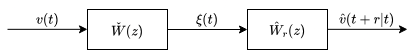
\includegraphics[width=0.75\linewidth]{images/wn.png}
\end{figure}